\documentclass[11pt,a4paper]{report}
\usepackage[textwidth=37em,vmargin=30mm]{geometry}
\usepackage{calc,xunicode,amsmath,amssymb,paralist,enumitem,tabu,booktabs,datetime2,xeCJK,xeCJKfntef,listings}
\usepackage{tocloft,fancyhdr,tcolorbox,xcolor,graphicx,eso-pic,xltxtra,xelatexemoji}

\newcommand{\envyear}[0]{2025}
\newcommand{\envdatestr}[0]{2025-09-06}
\newcommand{\envfinaldir}[0]{webdb/2025/20250906/final}

\usepackage[hidelinks]{hyperref}
\hypersetup{
    colorlinks=false,
    pdfpagemode=FullScreen,
    pdftitle={Web Digest - \envdatestr}
}

\setlength{\cftbeforechapskip}{10pt}
\renewcommand{\cftchapfont}{\rmfamily\bfseries\large\raggedright}
\setlength{\cftbeforesecskip}{2pt}
\renewcommand{\cftsecfont}{\sffamily\small\raggedright}

\setdefaultleftmargin{2em}{2em}{1em}{1em}{1em}{1em}

\usepackage{xeCJK,xeCJKfntef}
\xeCJKsetup{PunctStyle=plain,RubberPunctSkip=false,CJKglue=\strut\hskip 0pt plus 0.1em minus 0.05em,CJKecglue=\strut\hskip 0.22em plus 0.2em}
\XeTeXlinebreaklocale "zh"
\XeTeXlinebreakskip = 0pt


\setmainfont{Brygada 1918}
\setromanfont{Brygada 1918}
\setsansfont{IBM Plex Sans}
\setmonofont{JetBrains Mono NL}
\setCJKmainfont{Noto Serif CJK SC}
\setCJKromanfont{Noto Serif CJK SC}
\setCJKsansfont{Noto Sans CJK SC}
\setCJKmonofont{Noto Sans CJK SC}

\setlength{\parindent}{0pt}
\setlength{\parskip}{8pt}
\linespread{1.15}

\lstset{
	basicstyle=\ttfamily\footnotesize,
	numbersep=5pt,
	backgroundcolor=\color{black!5},
	showspaces=false,
	showstringspaces=false,
	showtabs=false,
	tabsize=2,
	captionpos=b,
	breaklines=true,
	breakatwhitespace=true,
	breakautoindent=true,
	linewidth=\textwidth
}






\newcommand{\coverpic}[2]{
    % argv: itemurl, authorname
    Cover photo by #2~~(\href{#1}{#1})
}
\newcommand{\makeheader}[0]{
    \begin{titlepage}
        % \newgeometry{hmargin=15mm,tmargin=21mm,bmargin=12mm}
        \begin{center}
            
            \rmfamily\scshape
            \fontspec{BaskervilleF}
            \fontspec{Old Standard}
            \fontsize{59pt}{70pt}\selectfont
            WEB\hfill DIGEST
            
            \vfill
            % \vskip 30pt
            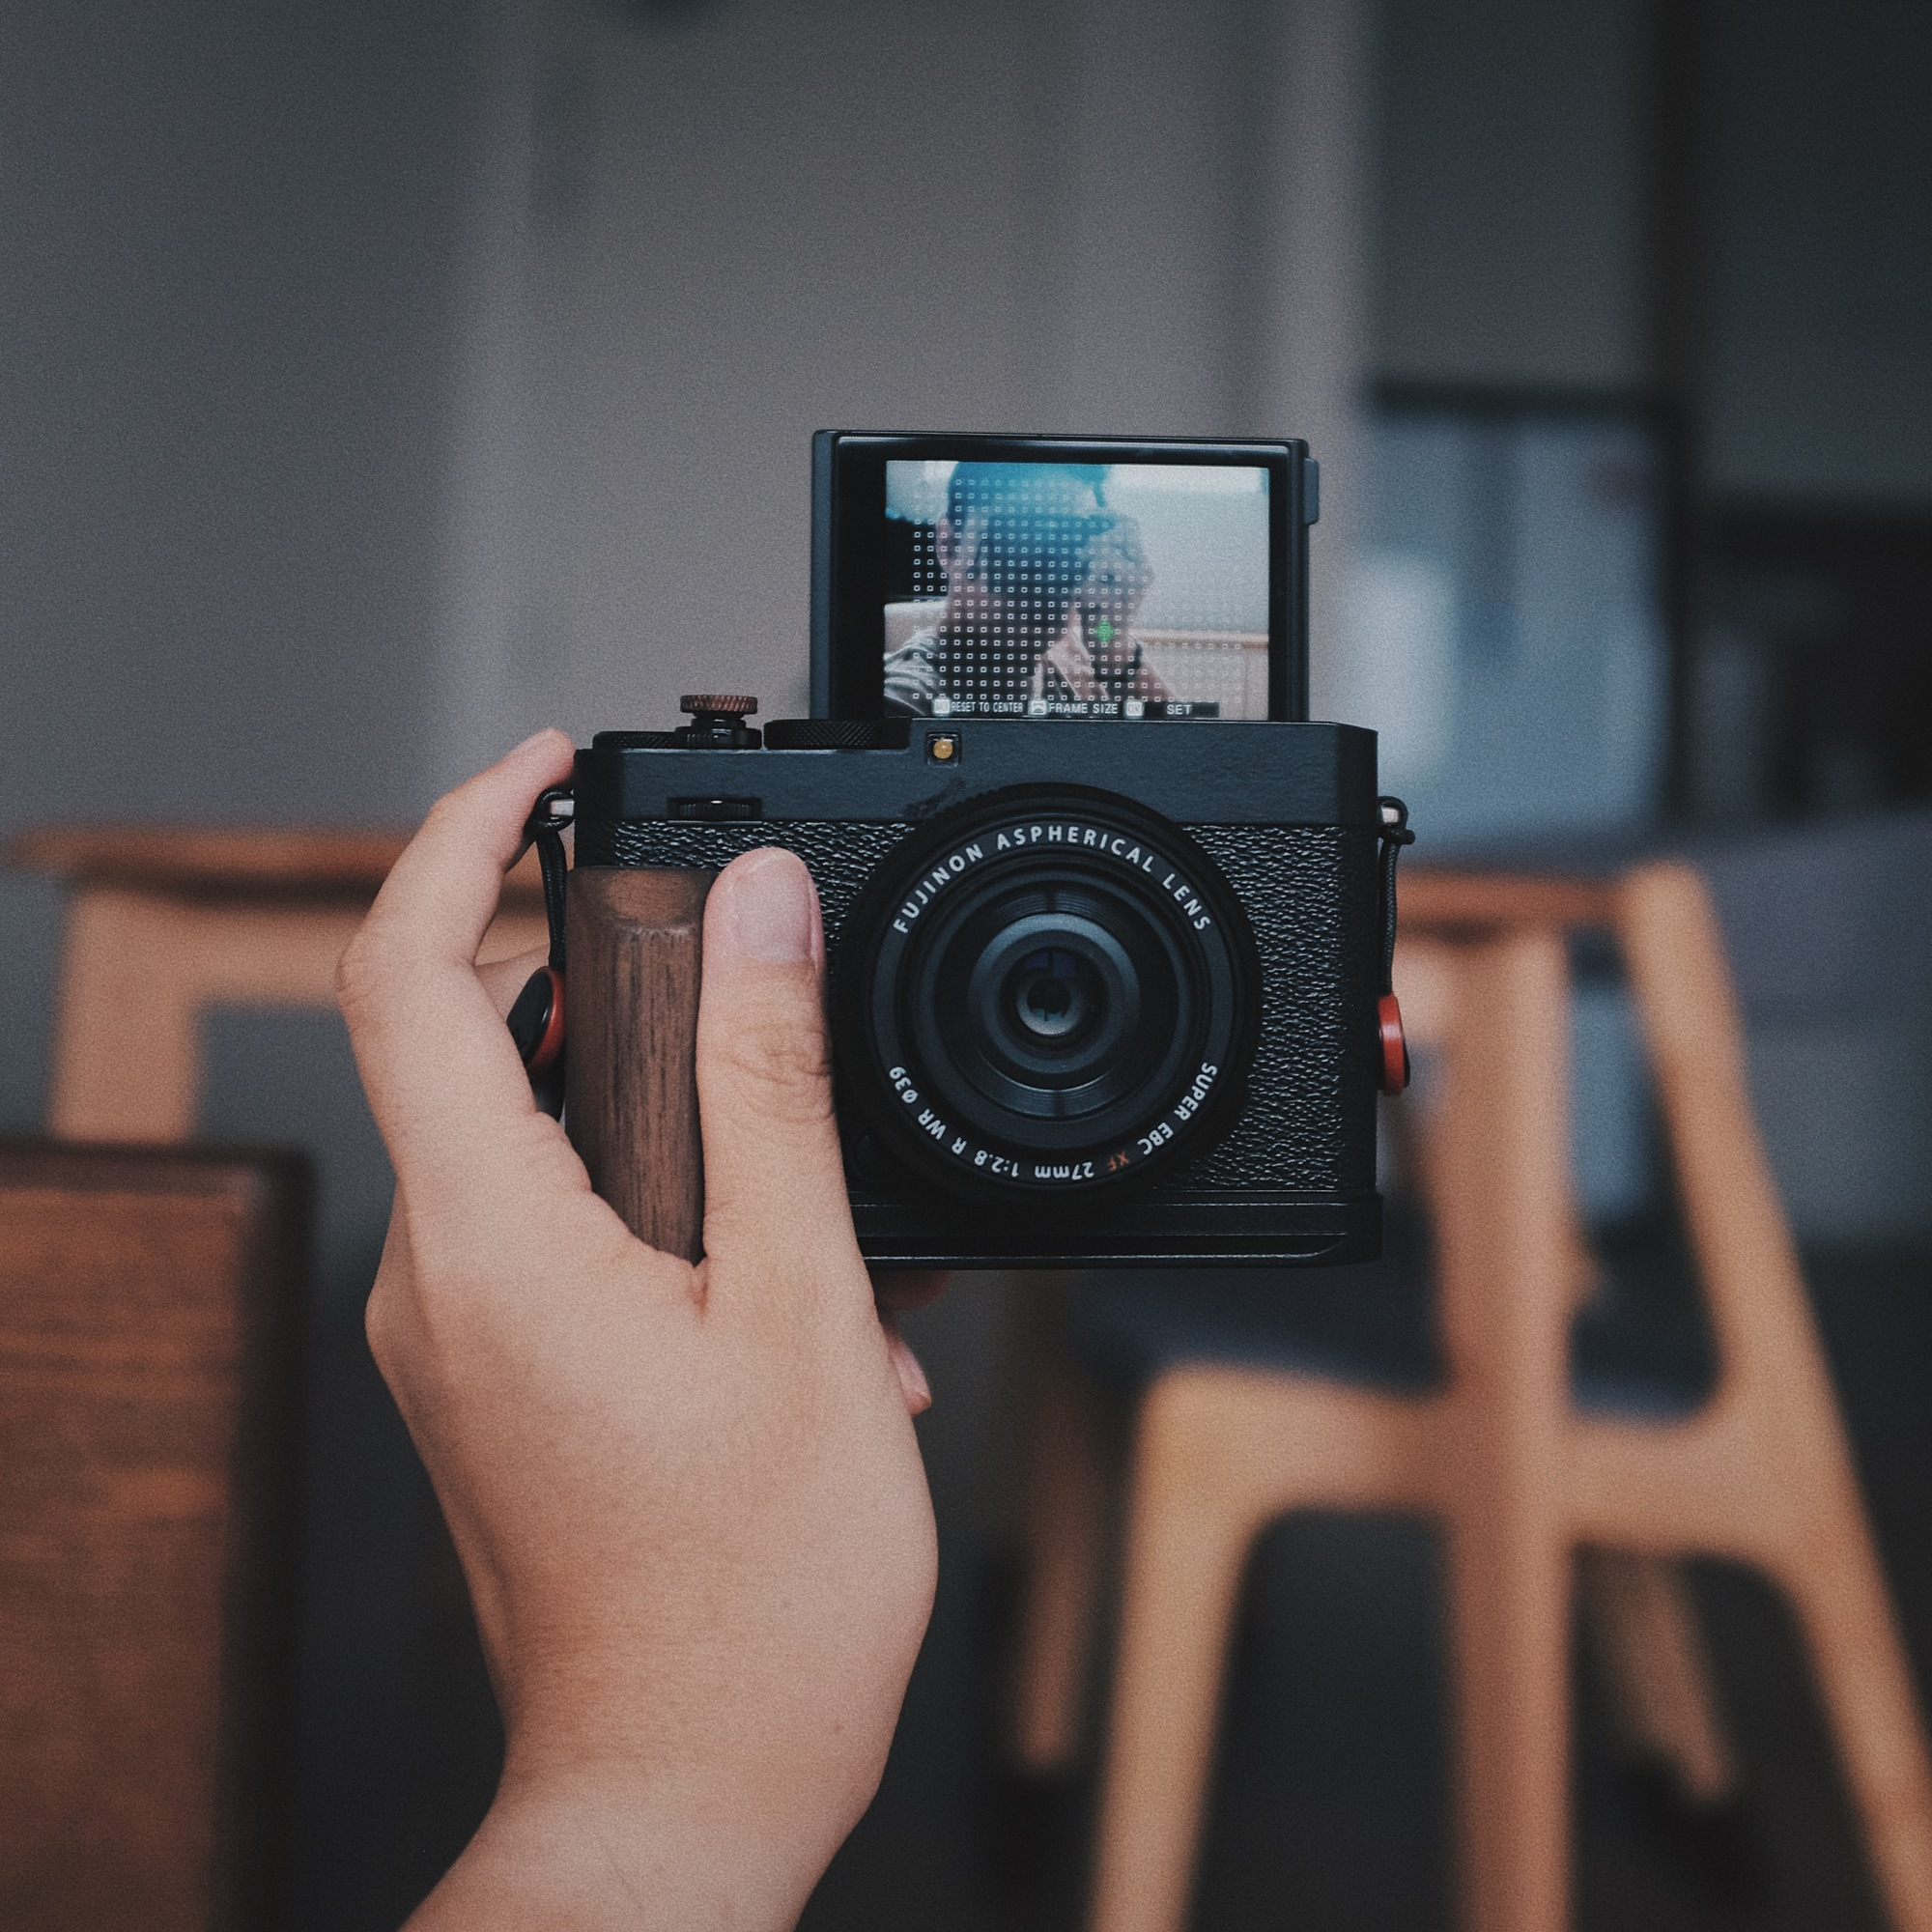
\includegraphics[width=\linewidth]{\envfinaldir/coverpic-prod.jpg}\par
            % \vskip 30pt
            \vfill

            \normalsize\rmfamily\scshape
            \copyright{} The Web Digest Project \hfill\large \envdatestr
        \end{center}
    \end{titlepage}
    % \restoregeometry
}
\newcommand{\simplehref}[1]{%
    \textcolor{blue!80!green}{\href{#1}{#1}}%
}
\renewcommand{\contentsname}{\center\Huge\sffamily\bfseries Contents\par\vskip 20pt}
\newcounter{ipartcounter}
\setcounter{ipartcounter}{0}
\newcommand{\ipart}[1]{
    % \vskip 20pt
    \clearpage
    \stepcounter{ipartcounter}
    \phantomsection
    \addcontentsline{toc}{chapter}{#1}
    % \begin{center}
    %     \Huge
    %     \sffamily\bfseries
    %     #1
    % \end{center}
    % \vskip 20pt plus 7pt
}
\newcounter{ichaptercounter}
\setcounter{ichaptercounter}{0}
\newcommand{\ichapter}[1]{
    % \vskip 20pt
    \clearpage
    \stepcounter{ichaptercounter}
    \phantomsection
    \addcontentsline{toc}{section}{\numberline{\arabic{ichaptercounter}}#1}
    \begin{center}
        \Huge
        \sffamily\bfseries
        #1
    \end{center}
    \vskip 20pt plus 7pt
}
\newcommand{\entrytitlefont}[1]{\subsection*{\raggedright\Large\sffamily\bfseries#1}}
\newcommand{\entryitemGeneric}[2]{
    % argv: title, url
    \parbox{\linewidth}{
        \entrytitlefont{#1}\par\vskip 5pt
        \footnotesize\ttfamily\mdseries
        \simplehref{#2}
    }\vskip 11pt plus 11pt minus 1pt
}
\newcommand{\entryitemGithub}[3]{
    % argv: title, url, desc
    \parbox{\linewidth}{
        \entrytitlefont{#1}\par\vskip 5pt
        \footnotesize\ttfamily\mdseries
        \simplehref{#2}\par\vskip 5pt
        \small\rmfamily\mdseries#3
    }\vskip 11pt plus 11pt minus 1pt
}
\newcommand{\entryitemAp}[3]{
    % argv: title, url, desc
    \parbox{\linewidth}{
        \entrytitlefont{#1}\par\vskip 5pt
        \footnotesize\ttfamily\mdseries
        \simplehref{#2}\par\vskip 5pt
        \small\rmfamily\mdseries#3
    }\vskip 11pt plus 11pt minus 1pt
}
\newcommand{\entryitemHackernews}[3]{
    % argv: title, hnurl, rawurl
    % \parbox{\linewidth}{
    %     \entrytitlefont{#1}\par\vskip 5pt
    %     \footnotesize\ttfamily\mdseries
    %     \simplehref{#3}\par
    %     \textcolor{black!50}{\href{#2}{#2}}
    % }\vskip 11pt plus 11pt minus 1pt
    \begin{minipage}{\linewidth}
            \entrytitlefont{#1}\par\vskip 5pt
            \footnotesize\ttfamily\mdseries
            \simplehref{#3}\par
            \textcolor{black!50}{\href{#2}{#2}}
    \end{minipage}\par\vskip 11pt plus 11pt minus 1pt
}







\begin{document}

\makeheader

\tableofcontents\clearpage




\ipart{Developers}
\ichapter{Hacker News}
\entryitemTwoLinks{Nest 1st gen and 2nd gen thermostats no longer supported from 10/25/2025}{https://news.ycombinator.com/item?id=45143879}{https://community.hubitat.com/t/nest-1st-gen-and-2nd-gen-thermostats-no-longer-supported-by-google-from-10-25-2025/152952}

\entryitemTwoLinks{I kissed comment culture goodbye}{https://news.ycombinator.com/item?id=45143077}{https://sustainableviews.substack.com/p/the-day-i-kissed-comment-culture}

\entryitemTwoLinks{Anthropic agrees to pay \$1.5B to settle lawsuit with book authors}{https://news.ycombinator.com/item?id=45142885}{https://www.nytimes.com/2025/09/05/technology/anthropic-settlement-copyright-ai.html?unlocked\_article\_code=1.jk8.bTTt.Zir9wmtPaTp2\&smid=url-share}

\entryitemTwoLinks{Making a font of my handwriting}{https://news.ycombinator.com/item?id=45141636}{https://chameth.com/making-a-font-of-my-handwriting/}

\entryitemTwoLinks{European Commission fines Google €2.95B over abusive ad tech practices}{https://news.ycombinator.com/item?id=45140730}{https://ec.europa.eu/commission/presscorner/detail/en/ip\_25\_1992}

\entryitemTwoLinks{South Korea: 'many' of its nationals detained in ICE raid on GA Hyundai facility}{https://news.ycombinator.com/item?id=45139954}{https://www.nbcnews.com/news/us-news/ice-hyundai-plant-georgia-enforcement-action-rcna229148}

\entryitemTwoLinks{Protobuffers Are Wrong (2018)}{https://news.ycombinator.com/item?id=45139656}{https://reasonablypolymorphic.com/blog/protos-are-wrong/}

\entryitemTwoLinks{A computer upgrade has shut down BART}{https://news.ycombinator.com/item?id=45139270}{https://www.bart.gov/news/articles/2025/news20250905}

\entryitemTwoLinks{Purposeful animations}{https://news.ycombinator.com/item?id=45139088}{https://emilkowal.ski/ui/you-dont-need-animations}

\entryitemTwoLinks{US economy added just 22,000 jobs in August, unemployment highest in 4 yrs}{https://news.ycombinator.com/item?id=45138703}{https://www.cnn.com/2025/09/05/economy/us-jobs-report-august-final}

\entryitemTwoLinks{Development speed is not a bottleneck}{https://news.ycombinator.com/item?id=45138156}{https://pawelbrodzinski.substack.com/p/development-speed-is-not-a-bottleneck}

\entryitemTwoLinks{I'm absolutely right}{https://news.ycombinator.com/item?id=45137802}{https://absolutelyright.lol/}

\entryitemTwoLinks{OpenAI eats jobs, then offers to help you find a new one at Walmart}{https://news.ycombinator.com/item?id=45137658}{https://www.theregister.com/2025/09/05/openai\_jobs\_board/}

\entryitemTwoLinks{I ditched Docker for Podman}{https://news.ycombinator.com/item?id=45137525}{https://codesmash.dev/why-i-ditched-docker-for-podman-and-you-should-too}

\entryitemTwoLinks{ML needs a new programming language – Interview with Chris Lattner}{https://news.ycombinator.com/item?id=45137373}{https://signalsandthreads.com/why-ml-needs-a-new-programming-language/}

\entryitemTwoLinks{Nepal moves to block Facebook, X, YouTube and others}{https://news.ycombinator.com/item?id=45137363}{https://www.aljazeera.com/news/2025/9/4/nepal-moves-to-block-facebook-x-youtube-and-others}

\entryitemTwoLinks{Interview with Japanese Demoscener 0b5vr}{https://news.ycombinator.com/item?id=45137245}{https://6octaves.com/2025/09/interview-with-demoscener-0b5vr.html}

\entryitemTwoLinks{I bought the cheapest EV, a used Nissan Leaf}{https://news.ycombinator.com/item?id=45136103}{https://www.jeffgeerling.com/blog/2025/i-bought-cheapest-ev-used-nissan-leaf}

\entryitemTwoLinks{SQL needed structure}{https://news.ycombinator.com/item?id=45135623}{https://www.scattered-thoughts.net/writing/sql-needed-structure/}

\entryitemTwoLinks{Age verification doesn't work}{https://news.ycombinator.com/item?id=45135529}{https://pornbiz.com/post/17/the\_scam\_of\_age\_verification}\ichapter{Phoronix}
\entryitemGeneric{\hskip 0pt{}New x86 Hardware Support \& Device Quirks Merged Ahead Of Linux 6.17-rc5}{https://www.phoronix.com/news/Linux-6.17-rc5-x86-Platform}

\entryitemGeneric{\hskip 0pt{}A First Look At Ubuntu 25.10 Performance On AMD Strix Halo / Framework Desktop}{https://www.phoronix.com/review/ubuntu-2510-strix-halo}

\entryitemGeneric{\hskip 0pt{}Wine 10.15 To Feature Initial Support For Using NTSYNC On Linux}{https://www.phoronix.com/news/Wine-10.15-With-NTSYNC}

\entryitemGeneric{\hskip 0pt{}Raspberry Pi Launches A 1TB SSD For \$70 USD}{https://www.phoronix.com/news/Raspberry-Pi-1TB-SSD}

\entryitemGeneric{\hskip 0pt{}Firefox Ending 32-bit Linux Support Next Year}{https://www.phoronix.com/news/Firefox-Ending-32-bit-Linux}

\entryitemGeneric{\hskip 0pt{}Xiaomi Redmibook Laptops To See Better Support With Linux 6.18}{https://www.phoronix.com/news/Redmibook-Keyboard-Linux-6.18}

\entryitemGeneric{\hskip 0pt{}Four Months Have Passed Since The Last AMDVLK Driver Release}{https://www.phoronix.com/news/AMDVLK-Four-Months-Go}

\entryitemGeneric{\hskip 0pt{}Linux Kernel Runtime Guard 1.0 Released For Security Vulnerability Exploit Detection}{https://www.phoronix.com/news/LKRG-1.0-Released}

\entryitemGeneric{\hskip 0pt{}Intel's Vulkan Linux Driver Finally Exposes VK\_EXT\_shader\_object}{https://www.phoronix.com/news/Intel-ANV-VK\_EXT\_shader\_object}


\ipart{Developers~~~~(zh-Hans)}
\ichapter{Solidot}
\entryitemGeneric{\hskip 0pt{}Mark Zuckerberg 起诉 Mark Zuckerberg}{https://www.solidot.org/story?sid=82236}

\entryitemGeneric{\hskip 0pt{}上厕所时用智能手机大幅增加痔疮风险}{https://www.solidot.org/story?sid=82235}

\entryitemGeneric{\hskip 0pt{}人工甜味剂与认知能力下降相关,相当于衰老 1.6 年}{https://www.solidot.org/story?sid=82234}

\entryitemGeneric{\hskip 0pt{}Anthropic 禁止中国控股公司使用 Claude}{https://www.solidot.org/story?sid=82233}

\entryitemGeneric{\hskip 0pt{}尼泊尔屏蔽大部分社媒平台}{https://www.solidot.org/story?sid=82232}

\entryitemGeneric{\hskip 0pt{}Atlassian 以 6.1 亿美元收购 Browser Company  }{https://www.solidot.org/story?sid=82229}

\entryitemGeneric{\hskip 0pt{}美国失业人数超过招聘人数}{https://www.solidot.org/story?sid=82228}

\entryitemGeneric{\hskip 0pt{}Fina Root CA 签发了三张 1.1.1.1 证书}{https://www.solidot.org/story?sid=82227}

\entryitemGeneric{\hskip 0pt{}《空洞骑士:丝之歌》上线,各大游戏平台服务器全部崩溃}{https://www.solidot.org/story?sid=82226}

\entryitemGeneric{\hskip 0pt{}森林砍伐让亚马孙雨林旱季降雨减少}{https://www.solidot.org/story?sid=82225}

\entryitemGeneric{\hskip 0pt{}瑞士发布了完整开源的大模型 Apertus}{https://www.solidot.org/story?sid=82224}

\entryitemGeneric{\hskip 0pt{}研究预测地球碳封存能力上限为 1.46 万亿吨}{https://www.solidot.org/story?sid=82223}

\entryitemGeneric{\hskip 0pt{}美国撤销台积电南京工厂的优待措施}{https://www.solidot.org/story?sid=82222}

\entryitemGeneric{\hskip 0pt{}照亮微塑料的细菌}{https://www.solidot.org/story?sid=82221}

\entryitemGeneric{\hskip 0pt{}太阳耀斑温度比以前认为的高出 6.5 倍}{https://www.solidot.org/story?sid=82220}

\entryitemGeneric{\hskip 0pt{}腾讯发布能从单张图像生成 3D 世界的模型 Voyager}{https://www.solidot.org/story?sid=82219}

\entryitemGeneric{\hskip 0pt{}Steam 每天增加 10 万新付费玩家}{https://www.solidot.org/story?sid=82218}

\entryitemGeneric{\hskip 0pt{}大模型让开源项目更容易受到类似 XZ 后门事件的攻击}{https://www.solidot.org/story?sid=82217}

\entryitemGeneric{\hskip 0pt{}研究证明电动汽车的温室气体排放低于燃油汽车}{https://www.solidot.org/story?sid=82216}

\entryitemGeneric{\hskip 0pt{}派拉蒙和动视联手制作《使命召唤》电影}{https://www.solidot.org/story?sid=82215}\ichapter{V2EX}
\entryitemGeneric{\hskip 0pt{}[云计算] 出租/出售美洲 arin ipv4 /24}{https://www.v2ex.com/t/1157421}

\entryitemGeneric{\hskip 0pt{}[加密货币] 「请教」合约,你们都盈利了嘛}{https://www.v2ex.com/t/1157420}

\entryitemGeneric{\hskip 0pt{}[汽车] 如何确定对面是开的远光}{https://www.v2ex.com/t/1157419}

\entryitemGeneric{\hskip 0pt{}[macOS] MacBook Pro M2 Max 只装了 5 个软件,每一两周就 kernal panic,报错都是 double free of xxx,怎么判断是软件还是硬件问题?}{https://www.v2ex.com/t/1157418}

\entryitemGeneric{\hskip 0pt{}[分享创造] 纯 flutter app 开发, web 入门级选手,做了 1 个练手网站}{https://www.v2ex.com/t/1157417}

\entryitemGeneric{\hskip 0pt{}[宽带症候群] 有没有 PPPoE 代拨转为 DHCP 下发 IP 的方法?}{https://www.v2ex.com/t/1157416}

\entryitemGeneric{\hskip 0pt{}[Android] Android 16 时尚是一个圆圈?}{https://www.v2ex.com/t/1157415}

\entryitemGeneric{\hskip 0pt{}[宽带症候群] 023 专线安装记录}{https://www.v2ex.com/t/1157414}

\entryitemGeneric{\hskip 0pt{}[分享发现] 用了三年的 iPhone 13 pm,自己换了电池}{https://www.v2ex.com/t/1157413}

\entryitemGeneric{\hskip 0pt{}[Google] 求助 谷歌账号异常,被停用,验证邮箱就是被停用的邮箱}{https://www.v2ex.com/t/1157412}

\entryitemGeneric{\hskip 0pt{}[程序员] 央视频的电视直播有没有电视端 app 啊}{https://www.v2ex.com/t/1157411}

\entryitemGeneric{\hskip 0pt{}[问与答] 程序员情侣在一起,是感情加倍还是矛盾加倍?}{https://www.v2ex.com/t/1157409}

\entryitemGeneric{\hskip 0pt{}[Arc] The Browser Company 被老牌协作厂商 Atlassian 收购, Arc 浏览器何去何从?}{https://www.v2ex.com/t/1157408}

\entryitemGeneric{\hskip 0pt{}[程序员] 手滑把服务器登陆信息随 log 贴给了 Cursor;除了修改登陆信息,还有别的补救方法吗?}{https://www.v2ex.com/t/1157407}

\entryitemGeneric{\hskip 0pt{}[推广] 37 岁程序员,未来 10 年还有希望吗?}{https://www.v2ex.com/t/1157406}

\entryitemGeneric{\hskip 0pt{}[分享创造] 现在还有人玩 morse code 么}{https://www.v2ex.com/t/1157405}

\entryitemGeneric{\hskip 0pt{}[推广] 深夜美食,麦当劳经典麦辣双人 8 件套}{https://www.v2ex.com/t/1157404}

\entryitemGeneric{\hskip 0pt{}[生活] 离婚对孩子的伤害有多大}{https://www.v2ex.com/t/1157402}

\entryitemGeneric{\hskip 0pt{}[程序员] 深度使用一段时间 Cursor 后, 分享一点我的实用小技巧}{https://www.v2ex.com/t/1157400}

\entryitemGeneric{\hskip 0pt{}[硬件] 3D 打印机 的电源/压 是否基本全球通用啊? 就是 220V 和 110V 都是一个款式的啊? 如手机充电器}{https://www.v2ex.com/t/1157398}

\entryitemGeneric{\hskip 0pt{}[Apple] iPhone 17 Air 国行疑似卡住了,大陆无首发}{https://www.v2ex.com/t/1157396}

\entryitemGeneric{\hskip 0pt{}[分享发现] 长时间来看,大模型会让我们越来越傻}{https://www.v2ex.com/t/1157395}

\entryitemGeneric{\hskip 0pt{}[美酒与美食] 迫……迫不了了,不知批萨好吃的点在哪,求推荐披萨,必胜客,达美乐等等}{https://www.v2ex.com/t/1157394}

\entryitemGeneric{\hskip 0pt{}[生活] 现在年龄大了, 特别想找人聊天...}{https://www.v2ex.com/t/1157393}

\entryitemGeneric{\hskip 0pt{}[硬件] 咨询万能 v 友,开机卡 vga,除了显卡,主板 pcie 外,还可能是什么问题}{https://www.v2ex.com/t/1157392}

\entryitemGeneric{\hskip 0pt{}[分享发现] 借助 Nano banana,我做了一个真实照片和动漫互转的网站}{https://www.v2ex.com/t/1157391}

\entryitemGeneric{\hskip 0pt{}[酷工作] [上海/100w - 200w/年] AI agent 开发 Leader 岗位}{https://www.v2ex.com/t/1157390}

\entryitemGeneric{\hskip 0pt{}[职场话题] [周末看法] 六年时光回看``996 是福报''是对是错?}{https://www.v2ex.com/t/1157388}

\entryitemGeneric{\hskip 0pt{}[程序员] 大模型学习路径求大佬指导!}{https://www.v2ex.com/t/1157387}

\entryitemGeneric{\hskip 0pt{}[iPhone] iPhone 双卡拨打紧急电话的 BUG 如何解决?}{https://www.v2ex.com/t/1157386}

\entryitemGeneric{\hskip 0pt{}[问与答] 暴汗体感游戏推荐}{https://www.v2ex.com/t/1157385}

\entryitemGeneric{\hskip 0pt{}[分享发现] Google 请每一位尊贵的 Chrome 用户吃 4G 的 Gemini}{https://www.v2ex.com/t/1157384}

\entryitemGeneric{\hskip 0pt{}[酷工作] [兼职招聘] 求浏览器插件前端工程师一枚(做一款插件,萌翻: AI 翻译/AI 词典)}{https://www.v2ex.com/t/1157383}

\entryitemGeneric{\hskip 0pt{}[分享发现] Perplexity Pro 一年会员免费送 这个羊毛大家薅了吗?}{https://www.v2ex.com/t/1157382}

\entryitemGeneric{\hskip 0pt{}[分享创造] 我做了一个 Nano Banana 提示词分享小站}{https://www.v2ex.com/t/1157381}

\entryitemGeneric{\hskip 0pt{}[问与答] 不懂就问,为什么总是能刷到问界车主在驾驶位睡觉打呼噜的视频}{https://www.v2ex.com/t/1157379}

\entryitemGeneric{\hskip 0pt{}[成都] 求,成都月子中心推荐}{https://www.v2ex.com/t/1157378}

\entryitemGeneric{\hskip 0pt{}[C++] [求助] Linux 系统下动态库卸载后全局变量未重置的问题}{https://www.v2ex.com/t/1157377}

\entryitemGeneric{\hskip 0pt{}[问与答] mac 上有什么 surge 平替}{https://www.v2ex.com/t/1157375}

\entryitemGeneric{\hskip 0pt{}[推广] 微众银行开户羊毛, 最高可领 400+}{https://www.v2ex.com/t/1157374}

\entryitemGeneric{\hskip 0pt{}[程序员] Sweep AI 是 idea 系唯一一个支持类似 cursor 的 next edit 功能的插件吗}{https://www.v2ex.com/t/1157373}

\entryitemGeneric{\hskip 0pt{}[问与答] 美团单车省流量方法?}{https://www.v2ex.com/t/1157372}

\entryitemGeneric{\hskip 0pt{}[问与答] 你们有没有遇到过大脑突然增强渲染现实的事情}{https://www.v2ex.com/t/1157370}

\entryitemGeneric{\hskip 0pt{}[分享发现] The Browser Company 被老牌协作软件厂商 Atlassian 收购, Arc 浏览器何去何从?}{https://www.v2ex.com/t/1157369}

\entryitemGeneric{\hskip 0pt{}[分享发现] 技术类语音识别(会议记录)的工具推荐和讨论}{https://www.v2ex.com/t/1157368}

\entryitemGeneric{\hskip 0pt{}[酷工作] [杭州 EFC] 招前端工程师}{https://www.v2ex.com/t/1157367}

\entryitemGeneric{\hskip 0pt{}[汽车] 车险维修代理,坑(大修)}{https://www.v2ex.com/t/1157366}

\entryitemGeneric{\hskip 0pt{}[JetBrains] IDEA 用了 184G 内存。。。再加上今年涨价,除了 VSCode 还有什么替换的 IDE 吗}{https://www.v2ex.com/t/1157365}

\entryitemGeneric{\hskip 0pt{}[奇思妙想] 分享一个网络开车的方法}{https://www.v2ex.com/t/1157364}

\entryitemGeneric{\hskip 0pt{}[问与答] 工行一直给我打骚扰电话,想换一家银行,求推荐。}{https://www.v2ex.com/t/1157363}


\ipart{Generic News}







\clearpage
\leavevmode\vfill
\footnotesize

Copyright \copyright{} 2023-2025 Neruthes and other contributors.

This document is published with CC BY-NC-ND 4.0 license.

The entries listed in this newsletter may be copyrighted by their respective creators.

This newsletter is generated by the Web Digest project.

The newsletters are also delivered via Telegram channel \CJKunderline{\href{https://t.me/webdigestchannel}{https://t.me/webdigestchannel}}.\\
RSS feed is available at \CJKunderline{\href{https://webdigest.pages.dev/rss.xml}{https://webdigest.pages.dev/rss.xml}}.

This newsletter is available in PDF at
\CJKunderline{\href{https://webdigest.pages.dev/}{https://webdigest.pages.dev/}}.

The source code being used to generate this newsletter is available at\\
\CJKunderline{\href{https://github.com/neruthes/webdigest}{https://github.com/neruthes/webdigest}}.

This newsletter is also available in
\CJKunderline{\href{http://webdigest.pages.dev/readhtml/\envyear/WebDigest-20250906.html}{HTML}} and
\CJKunderline{\href{https://github.com/neruthes/webdigest/blob/master/markdown/\envyear/WebDigest-20250906.md}{Markdown}}.


\coverpic{https://unsplash.com/photos/pink-umbrella-hanging-against-brick-wall-\_QIwNf5ks-o}{Brother Yoon}


\end{document}
